\documentclass[letterpaper]{article} % DO NOT CHANGE THIS
\usepackage[submission]{aaai2027}  % DO NOT CHANGE THIS
\usepackage[hyphens]{url}  % DO NOT CHANGE THIS
\usepackage{graphicx} % DO NOT CHANGE THIS
\urlstyle{rm} % DO NOT CHANGE THIS
\def\UrlFont{\rm}  % DO NOT CHANGE THIS
\usepackage{natbib}  % DO NOT CHANGE THIS AND DO NOT ADD ANY OPTIONS TO IT
\usepackage{caption} % DO NOT CHANGE THIS AND DO NOT ADD ANY OPTIONS TO IT
\frenchspacing  % DO NOT CHANGE THIS
\usepackage{algorithm}
\usepackage{algorithmic}
\usepackage{booktabs}

\hyphenation{}

\pdfinfo{
/TemplateVersion (2027.1)
}

\setcounter{secnumdepth}{0}

\title{Behavior-Assisted Recovery of Protected System Prompts: A Mechanism-Level Study}
\author{Anonymous Submission}
\affiliations{}

\begin{document}

\maketitle

\begin{abstract}
Prompt-protection mechanisms hide prompt text or representations while preserving model utility.  We study whether the preserved behavior itself can support recovery of hidden prompt structure.  We introduce a multi-evidence recovery pipeline that combines a mechanism-inspired protected representation, auxiliary prompt metadata, and six task-matched input--output traces.  A Qwen3-32B recovery model is adapted with QLoRA to predict six structured fields: role/persona, task, format, constraints, context, and tool/protocol.  We evaluate eight mechanism-aligned protection transformations over six prompt categories, with 100 prompts per category and 960 prompt-level held-out evaluations in total.

In this mechanism-level benchmark, mean Text F1 ranges from 0.380 to 0.679, ROUGE-L F1 ranges from 0.312 to 0.606, and behavior-level Utility F1 ranges from 0.361 to 0.433 across protection transformations.  Pr$\epsilon\epsilon$mpt-style sanitization gives the highest Text F1 (0.679) and ROUGE-L F1 (0.606), while InferDPT-style token perturbation gives the highest Utility F1 (0.433).  Recovery is also category-dependent: role/persona and context expose repeated behavioral signals more often, whereas constraints and tool protocols require more targeted probes.  The study motivates a privacy criterion that evaluates behaviorally useful prompt recovery in addition to direct text exposure.
\end{abstract}

\section{Introduction}

Private system prompts encode roles, task logic, output schemas, safety rules, background knowledge, and tool protocols.  In cloud-hosted inference, these instructions must affect a remote model without being exposed more than necessary.  Recent defenses address this problem through token perturbation, representation noise, prompt confusion, sanitization, symbolic rewriting, confidential execution, and cloud--edge collaboration~\citep{mai2026confusionprompt,tong2025inferdpt,mai2024split,chowdhury2025preempt,lin2024emojiprompt,lee2024confidential,zhan2026prism}.  Although their mechanisms differ, they share a difficult objective: conceal the prompt while retaining the behavior that makes the prompt useful.

Existing evaluations mainly measure representation privacy or downstream task utility.  These tests do not fully answer whether the instruction encoded in protected-system behavior remains inferable.  Exact token recovery is also too narrow a security criterion: recovering a hidden role, decision rule, output schema, or tool protocol may be sufficient to reproduce useful behavior without reproducing the original wording.  Prompt extraction and prompt stealing research demonstrates that generated outputs can reveal prompt information~\citep{zhang2024effective,sha2024promptstealing,hui2024pleak,deng2024promptleakage,das2025spe}, but protected-prompt settings have not been evaluated under one common structure-recovery pipeline.

We study this gap with a mechanism-level common-interface benchmark.  A multi-evidence recovery procedure predicts a structured description of the hidden prompt and converts the recovered fields into an executable system prompt.  We evaluate both textual overlap and functional similarity.  The precise observable view and access assumptions are defined only in the Threat Model.

Our contributions are as follows:
\begin{itemize}
    \item We formulate residual prompt leakage as recovery of a six-field latent instruction from server-visible evidence and prompt-induced behavior.
    \item We specify a symbolic threat model and a reproducible multi-evidence recovery pipeline, including matched-probe construction, structured targets, a QLoRA recovery model, and continuous text- and behavior-level evaluation metrics.
    \item We reproduce the soft-prompt foundation experiment and record its obfuscation utility, direct extraction, projection, and optimization-based recovery results.
    \item We build a category-balanced benchmark covering eight mechanism-inspired protection transformations, six prompt categories, and 4,800 category-instance--transformation pairs.
    \item We report Text F1, ROUGE-L F1, and Utility F1 for every transformation and show that average Utility F1 remains between 0.361 and 0.433 in the common-interface benchmark.
\end{itemize}

\section{Related Work}

\subsection{Prompt Privacy and Protected LLM Inference}

Prompt privacy differs from training-data privacy because the sensitive object is an inference-time instruction and its context~\citep{edemacu2024privacy}.  Privacy in language also cannot be reduced to one narrow token-level definition~\citep{brown2022privacymeaning}.  Prompt Obfuscation replaces readable instructions with optimized continuous vectors~\citep{pape2025promptobfuscation}.  Token-level local differential privacy protects natural language through calibrated substitutions~\citep{yue2021santext,chen2023custext}, while representation-level approaches perturb embeddings or pretrained representations~\citep{qu2021privacybert,zhou2023textobfuscator}.  Recent prompt-specific systems extend these ideas with confusion, token perturbation, split inference, or private prompt optimization~\citep{mai2026confusionprompt,tong2025inferdpt,mai2024split,hong2024dpopt}.  Their common design tension is that stronger perturbation hides more input information but can also remove the semantics required for useful inference.

\subsection{Prompt Sanitization, Symbolic Obfuscation, and Confidential Prompting}

Sanitization and symbolic obfuscation modify the prompt surface while preserving task cues.  Pr$\epsilon\epsilon$mpt combines typed protection mechanisms for sensitive spans~\citep{chowdhury2025preempt}, and EmojiPrompt uses linguistic and non-linguistic symbols to reduce direct readability~\citep{lin2024emojiprompt}.  Other systems alter the execution architecture: Confidential Prompting uses protected prompt execution~\citep{lee2024confidential}, NOIR uses randomized tokenization for protected code-generation workflows~\citep{nguyen2026noir}, and PRISM routes prompts between local and cloud paths according to privacy risk~\citep{zhan2026prism}.  Because these systems expose different interfaces, security claims depend on the observable artifact; we formalize that artifact in the Threat Model.

Table~\ref{tab:related_families} summarizes the literature by protected surface and residual signal rather than listing papers only by name.

\begin{table}[t]
\centering
\small
\setlength{\tabcolsep}{3pt}
\begin{tabular}{p{0.20\columnwidth}p{0.30\columnwidth}p{0.39\columnwidth}}
\toprule
Family & Representative work & Signal retained for utility \\
\midrule
Confusion & ConfusionPrompt & Genuine instruction fragments \\
Token privacy & InferDPT, Pr$\epsilon\epsilon$mpt & Task words, types, placeholders \\
Representation privacy & Split-N-Denoise, TextObfuscator & Semantic embedding geometry \\
Private prompting & DP-OPT, Confidential Prompting & Transferable or virtual prompt signal \\
Symbolic rewriting & EmojiPrompt, NOIR & Encoded task and format structure \\
Cloud--edge routing & PRISM & Cloud-visible semantic sketch \\
\bottomrule
\end{tabular}
\caption{Prompt-protection families and the information they retain to preserve utility.  Retained signal is a potential recovery channel, not proof that an original system is broken.}
\label{tab:related_families}
\end{table}

\subsection{Prompt Leakage, Prompt Stealing, and System Prompt Extraction}

Prompt extraction attacks recover hidden instructions through direct elicitation, adversarial optimization, or multi-turn interaction~\citep{zhang2024effective,hui2024pleak,deng2024promptleakage,das2025spe}.  Prompt stealing further shows that output behavior can reveal prompt properties even without verbatim disclosure~\citep{sha2024promptstealing}.  Our study differs in its protected-input setting and in treating behavior-level imitation as a first-class outcome.  The open question is not only whether a prompt can be printed, but whether a transformed prompt still exposes enough structure to recreate its function.

\section{System Model and Problem Definition}

\subsection{System Model}

Let the private system prompt be a random variable \(P\in\mathcal{P}\).  A trusted client-side protection component produces an intermediate protected state
\[
H=T(P;\xi_T),
\]
where \(\xi_T\) denotes mechanism randomness, and releases a cloud-visible payload \(Z=\Pi(H)\).  The intermediate state \(H\) and the transformation randomness remain inside the client trust boundary.  The cloud inference service, parameterized by \(\theta_M\), receives \((Z,X)\) and returns
\[
Y\sim P_{M_{\theta_M}}(\cdot\mid Z,X).
\]
Thus, \(H\) is not a hidden state inside the cloud model: it is a client-local state used to construct the payload that the cloud actually executes.  A useful protection layer aims to preserve output behavior,
\[
\mathbb{E}_{X\sim\mathcal{D}_P}[\operatorname{sim}(M_{\theta_M}(P,X),M_{\theta_M}(Z,X))]\geq\tau_u,
\]
while reducing direct exposure of the original representation.  The prompt's behaviorally relevant structure is
\[
S=s(P)=(S_r,S_t,S_f,S_c,S_k,S_q),
\]
where the fields denote role/persona, task, format, constraints, context, and tool/protocol.  Recovery targets \(S\), rather than requiring exact inversion of \(T\) or exact equality with \(P\).

\subsection{Threat Model}

The adversary \(\mathcal{A}\) is a service-operator adversary: it represents either the cloud inference provider or an entity that compromises the provider's logging and control plane after the client has transmitted \(Z\).  It observes all server-side information, including the model parameters \(\theta_M\), the received payload \(Z\), queries, and responses.  It can replay a stored payload through at most \(q\) chosen diagnostic queries.  This is therefore a bounded chosen-query, server-visible attack rather than a query-only external attack or a purely passive honest-but-curious observer.

Let \(A\) denote auxiliary metadata and \(D_{\mathrm{aux}}\) an auxiliary supervised corpus.  For queries \(X_{1:q}\) and responses \(Y_{1:q}\), define the server-side transcript and complete recovery view as
\[
W_q=(Z,X_{1:q},Y_{1:q}), \qquad V_q=(D_{\mathrm{aux}},A,\theta_M,W_q).
\]
The attacker \(\mathcal{A}\) is restricted to \(V_q\) and outputs
\[
(\hat{S},\hat{P})=\mathcal{A}(V_q),
\]
where \(\hat{S}\) estimates the latent fields and \(\hat{P}\) is an executable prompt.  No server-side state is hidden from this adversary.  What remains unavailable is the client-side private prompt \(P\), intermediate state \(H\), and mechanism randomness \(\xi_T\).  The attacker may choose \(X_i\) according to the preceding transcript, but it may not compromise the client trust boundary, bypass \(\Pi\), or exceed \(q\).  This definition fixes one real-world role and one observable interface across transformations.

\begin{figure*}[t]
    \centering
    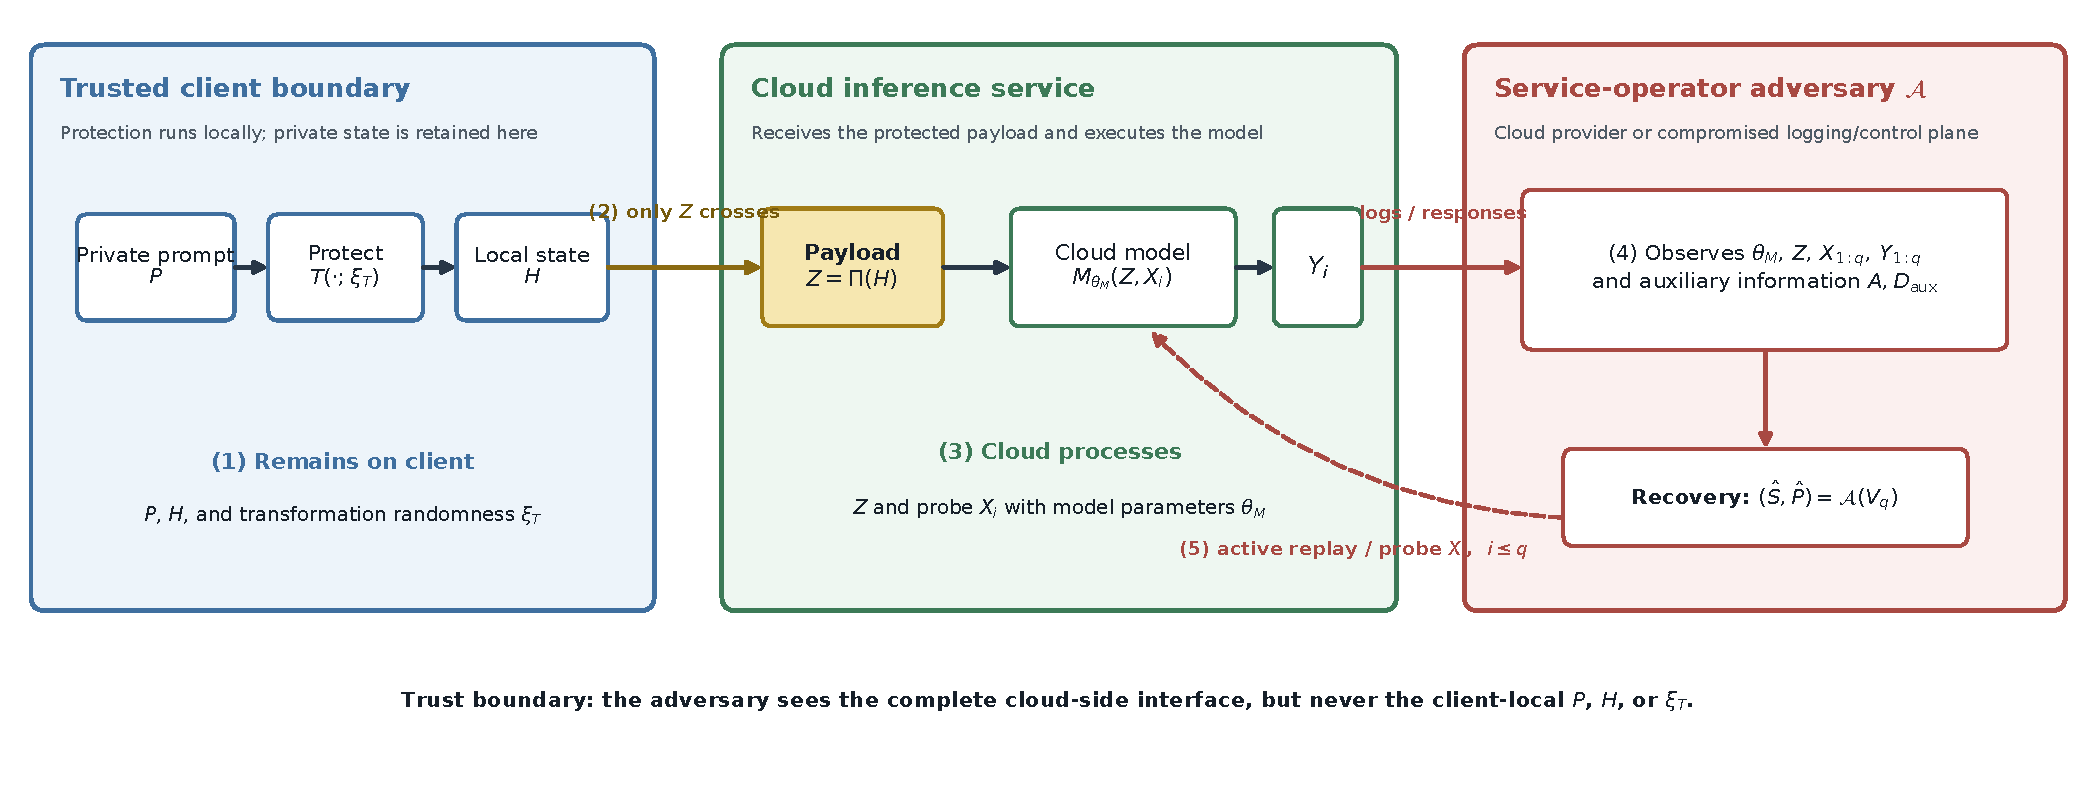
\includegraphics[width=\textwidth]{figures/threat_model_mapping.pdf}
    \caption{System boundary and adversary mapping.  (1) The trusted client retains \(P\), \(H\), and \(\xi_T\).  (2) Only the protected payload \(Z=\Pi(H)\) is transmitted.  (3) The cloud model processes \((Z,X_i)\).  (4) The service-operator adversary observes the model, payload, queries, responses, and auxiliary information.  (5) It may replay the stored payload with at most \(q\) active probes.  The adversary is therefore the cloud operator or a compromise of its control plane, not an external query-only API observer.}
    \label{fig:threat_model_mapping}
\end{figure*}

We measure residual information beyond the auxiliary side information by
\[
\mathcal{L}_q=I(S;W_q\mid A,D_{\mathrm{aux}},\theta_M)
=I(S;Z,X_{1:q}\mid A,D_{\mathrm{aux}},\theta_M)
+I(S;Y_{1:q}\mid Z,X_{1:q},A,D_{\mathrm{aux}},\theta_M).
\]
Under the stated service interface, execution satisfies the Markov relation \(S\rightarrow Z\rightarrow Y\) conditional on \((X,\theta_M)\).  If generation is deterministic, or uses randomness independent of \(S\) once \((Z,X,\theta_M)\) is fixed, then
\[
I(S;Y_{1:q}\mid Z,X_{1:q},A,D_{\mathrm{aux}},\theta_M)=0.
\]
Consequently, the responses are not claimed to create additional Shannon information beyond the complete server-visible payload.  They are operational features that can make the effect of \(Z\) easier for a computationally bounded recovery procedure to decode.  If a deployed service uses any additional prompt-dependent server state, that state must be included in \(Z\) because it is visible to the service-operator adversary.  Our experiments do not estimate \(\mathcal{L}_q\); they measure the operational recoverability of \(S\) and the behavioral utility of \(\hat{P}\) from \(V_q\).

\section{Recovery Method and Experimental Design}

\subsection{Soft-Prompt Foundation Reproduction}

We first reproduce the core experiment of Prompt Obfuscation~\citep{pape2025promptobfuscation}.  Llama-3.1-8B-Instruct is loaded in 4-bit precision and evaluated on 800 TruthfulQA inputs with two system-prompt styles, pirate and robot.  Each readable prompt initializes a ten-vector soft prompt, which is optimized with window size 5, learning rate 0.01, ten optimization iterations, and a 15-token output budget.  For pirate style, obfuscated-versus-original outputs reach BERTScore 0.9122, SacreBLEU 49.20, and ROUGE-L 0.4606; for robot style, the corresponding values are 0.9302, 49.23, and 0.5266.  These values closely match rerunning the readable prompt under a different generation seed.

The reproduction also covers the paper's three recovery evaluations.  Across 105 direct extraction queries, the readable prompt produces 33 exact and 41 near-exact extractions, whereas the ten-vector prompt produces zero in both groups; mean ROUGE-L recall falls from 0.4985 to 0.1293.  Nearest-token projection reaches Jaccard 0.064.  Optimization-based soft recovery preserves pirate-style output behavior at BERTScore 0.9122 but has Jaccard 0.000, while hard recovery reaches Jaccard 0.077, close to the published 0.084.  We report this foundation reproduction separately because it uses two style prompts and the original paper's metrics; the eight-condition benchmark below uses six category-balanced prompt sets and the common Text-F1/Utility-F1 protocol.

\subsection{Mechanism-Aligned Protection Benchmark}

We construct 100 prompt instances for each of six categories: Role/Persona, Task Instruction, Format Specification, Constraints, Context Knowledge, and Tool/Protocol.  The prompt pool combines three previously classified collections.  We first select prompts whose dominant six-dimensional label matches the target category.  Oversized categories are downsampled in proportion to source counts; undersized categories are filled by descending score on the corresponding dimension.  Selection is deterministic with seed 42.  A prompt may contain several instruction types and may enter more than one category set during score-based filling.  The 600 category instances contain 522 unique prompt IDs; applying eight transformations produces 4,800 category-instance--transformation pairs.

The transformations are \emph{mechanism-inspired benchmark abstractions}.  They isolate a central protection idea in a common text-and-sketch interface: mixed genuine and pseudo fragments for ConfusionPrompt; token substitutions for InferDPT; noisy embedding identifiers for Split-N-Denoise; virtual prompt sets for Confidential Prompting; randomized token IDs for NOIR; emoji-coded tokens for EmojiPrompt; noisy keyword votes for DP-OPT; and typed placeholders for Pr$\epsilon\epsilon$mpt.  These transformations do not reproduce complete cryptographic, differential-privacy, trusted-execution, or cloud--edge protocols.  Consequently, method names are always reported with the suffix ``-style,'' and the results compare benchmark transformations rather than the security guarantees of the original systems.

\begin{table*}[t]
\centering
\small
\setlength{\tabcolsep}{4pt}
\begin{tabular}{p{0.16\textwidth}p{0.34\textwidth}p{0.40\textwidth}}
\toprule
Condition & Common-interface artifact & End-to-end reproduction target \\
\midrule
ConfusionPrompt-style & Shuffled genuine and pseudo prompt fragments & Published decomposition, encryption, and private recombination \\
InferDPT-style & Locally substituted tokens plus a weak keyword sketch & Published LDP sampler and output extraction module \\
Split-N-Denoise-style & Noisy embedding-like identifiers & Split execution, calibrated noise, and learned denoiser \\
Confidential Prompting-style & Four virtual prompt strings & Protected hardware path and complete execution protocol \\
NOIR-style & Randomized token IDs with placeholders & Learned vocabulary and protected code workflow \\
EmojiPrompt-style & Deterministic emoji-coded tokens and weak keywords & Generative obfuscator and published decoding protocol \\
DP-OPT-style & Generic private template with noisy keyword votes & Private ensemble optimization and DP accounting \\
Pr$\epsilon\epsilon$mpt-style & Prompt text with typed placeholders & Complete sanitizer and type-specific protection mechanism \\
\bottomrule
\end{tabular}
\caption{The reported common-interface conditions and the components required for an end-to-end reproduction of each protection family.}
\label{tab:benchmark_scope}
\end{table*}

\subsection{Benchmark Transformation Parameters}

The common-interface transformations use a local random generator keyed by seed 42, method, category, and prompt ID.  ConfusionPrompt-style mixes up to six sentence-level prompt fragments with three to six category-matched pseudo fragments.  InferDPT-style always replaces words in a fixed sensitive-word map; for other lexical tokens longer than three characters, it uses prefix truncation with probability 0.25, a hashed identifier with probability 0.25, first/last-character masking with probability 0.20, and otherwise retains the token.  Split-N-Denoise-style maps up to 28 content words to a partial-word identifier with probability 0.45 and to an embedding-like hash otherwise.  Confidential-Prompting-style constructs four virtual strings, each combining a pseudo instruction with at most three prompt keywords.  NOIR-style maps the first 90 lexical tokens to a 5,000-symbol ID space while retaining placeholders.  EmojiPrompt-style maps the first 140 tokens through SHA-256 into 20 emoji symbols and a three-digit suffix, retains placeholders, and provides a 12-keyword sketch.  DP-OPT-style considers up to 20 keywords, drops each with probability 0.25, masks a retained vote with probability 0.35, and keeps at most ten votes.  Pr$\epsilon\epsilon$mpt-style replaces role, task, format, constraint, context, tool, entity, and numeric spans with typed placeholders and retains the first 12 sentence chunks.  All generated protected artifacts and traces are serialized before training; these serialized recovery-input files are the canonical inputs for the reported benchmark.

\subsection{End-to-End Reproduction Protocol}

For a protection method \(d\), a complete system reproduction instantiates the published transform \(T_d\), interface \(\Pi_d\), execution model \(M_d\), and privacy configuration \(\lambda_d\).  Before recovery evaluation, the implementation must reproduce the original paper's reported utility and privacy metrics under its stated data and model configuration, within a tolerance fixed before testing.  Recovery evidence is then constructed only from
\[
Z_d=\Pi_d(T_d(P;\lambda_d)),\qquad
Y_{d,i}\sim P_{M_d}(\cdot\mid T_d(P;\lambda_d),X_i),
\]
using the channels permitted by the Threat Model.  Evidence probes and final evaluation probes must be disjoint, and method-specific parameters---including privacy budgets, noise scales, sanitization rules, local/cloud components, tokenizers, checkpoints, and decoding settings---must be logged.  This protocol defines the end-to-end reproduction track; the numerical results below are produced by the fully specified common-interface track in Table~\ref{tab:benchmark_scope}.

\subsection{Recovery Evidence and Matched Probes}

For each target, the recovery input contains: (1) prompt ID, source label, paper title, and six category scores; (2) the mechanism-inspired protected text; (3) a semantic sketch and a short description of the visible evidence; and (4) six behavior traces.  In the notation of the Threat Model, these instantiate \(A\), \(Z\), and \((X_{1:q},Y_{1:q})\) with \(q=6\).

A probe is \emph{matched} when it is drawn from the cached test-input set associated with the same original prompt and follows that prompt's task format.  For example, a classification prompt receives classification-shaped inputs rather than generic questions.  For each matched probe \(x_i\), the evidence contains \((x_i,y_i)\).  In the current benchmark, \(y_i=M(p,x_i)\), the cached original-prompt output, is used as a high-utility proxy for \(M(T(p),x_i)\).  This design asks whether an ideally utility-preserving transformation would still leave recoverable structure; it does not measure the actual utility of an end-to-end defense implementation.

\subsection{Structured Targets and Recovery Model}

Reference targets are deterministic six-field JSON objects.  Sentences from the original prompt are assigned by lexical rules to role, task, format, constraints, context, and tool/protocol; unclear fields are empty.  Because one sentence can match multiple rules, these are automatically generated supervision labels rather than human-verified gold annotations.

For every protection-style/category pair, we shuffle prompt IDs with seed 42 and train on 80 prompts, leaving 20 for testing.  The recovery model is Qwen3-32B~\citep{yang2025qwen3} loaded in 4-bit NF4 with double quantization.  QLoRA~\citep{dettmers2023qlora} adapters use rank 16, scaling factor 32, dropout 0.05, and attention plus MLP projection modules.  Training uses five epochs, batch size 2, gradient accumulation 4, learning rate \(2\times10^{-4}\), and maximum sequence length 2,048.  At test time, greedy decoding produces one six-field JSON object with at most 180 new tokens.  We train 48 adapters in total, one for each of eight transformations and six categories.

\begin{algorithm}[t]
\caption{Multi-Evidence Structured Prompt Recovery}
\label{alg:recovery}
\begin{algorithmic}[1]
\REQUIRE Auxiliary prompt pairs \(D_{\mathrm{aux}}\), held-out prompt \(p\), transformation \(T\), query budget \(n=6\)
\STATE Build visible protected evidence \(z\leftarrow\Pi(T(p))\)
\STATE Select matched inputs \(X\leftarrow\{x_i\}_{i=1}^{n}\) from the prompt's cached task inputs
\STATE Collect proxy traces \(B\leftarrow\{(x_i,M(p,x_i))\}_{i=1}^{n}\)
\STATE Fine-tune \(R_\theta\) on 80 auxiliary prompts for the same transformation and category
\STATE Predict six fields \(\hat{S}\leftarrow R_\theta(z,B,\text{metadata})\)
\STATE Concatenate nonempty fields to obtain executable prompt \(\hat{P}\)
\STATE Evaluate text overlap and behavior similarity on the 20 held-out prompt IDs
\RETURN \(\hat{S},\hat{P}\), Text F1, ROUGE-L F1, Utility F1
\end{algorithmic}
\end{algorithm}

\subsection{Evaluation Metrics}

Text F1 is bag-of-token overlap between the recovered JSON and the reference JSON; ROUGE-L F1 measures longest-common-subsequence overlap~\citep{lin2004rouge}.  For two token sequences \(a\) and \(b\), let \(o(a,b)\) be their multiset token overlap.  Token precision is \(o(a,b)/|a|\), token recall is \(o(a,b)/|b|\), and Token F1 is their harmonic mean.  It does not use token position and is not a semantic-similarity metric.

To compute Utility F1, we concatenate the recovered nonempty fields into \(\hat{p}\), run Llama-3.1-8B-Instruct~\citep{grattafiori2024llama3} with \(\hat{p}\) on each matched input, and compare its output with the cached original-prompt output using Token F1.  For prompt \(p\), the prompt-level behavior score is the mean over six probe outputs:
\[
\operatorname{UtilityF1}(\hat{p},p)=\frac{1}{6}\sum_{i=1}^{6}\operatorname{TokenF1}(M(\hat{p},x_i),M(p,x_i)).
\]
Thus, Token F1 is the common overlap function rather than a separate experiment-level metric.  Text F1 applies it to prompt representations, whereas Utility F1 applies it to model outputs produced on matched probes.  Text F1 measures wording recovery, ROUGE-L F1 additionally reflects sequential overlap, and Utility F1 is an operational measure of behavioral imitation.  We retain the continuous scores instead of converting Utility F1 into a binary success decision at an arbitrary threshold.  Because evidence and evaluation queries overlap in the reported common-interface experiment, Utility F1 measures in-distribution reconstruction.

\subsection{Reproduction Record for the Reported Prompt Experiment}

Each of the 48 method--category datasets contains 100 prompt IDs.  Across the six category sets, 102 instances come from the combined prior collection, 189 from the 335-prompt batch, and 309 from the 417-prompt batch.  Dominant-label selection supplies 99, 100, 88, 27, 61, and 51 instances for Role, Task, Format, Constraints, Context, and Tool, respectively; score-based filling supplies the remainder.  Seed 42 shuffles each method--category dataset into 80 auxiliary training prompts and 20 prompt-disjoint test prompts, yielding 960 held-out category-transformation evaluations.  Every recovery input contains six matched traces.  Qwen3-32B~\citep{yang2025qwen3} is loaded with 4-bit NF4 double quantization and adapted with QLoRA~\citep{dettmers2023qlora}: rank 16, scaling 32, dropout 0.05, attention and MLP projection targets, five epochs, batch size 2, gradient accumulation 4, learning rate \(2\times10^{-4}\), and maximum length 2,048.  Greedy recovery decoding is capped at 180 new tokens.  Utility evaluation uses Llama-3.1-8B-Instruct~\citep{grattafiori2024llama3} and the same six matched inputs.  Text F1, ROUGE-L F1, and prompt-level Utility F1 are aggregated first within each category and then by transformation.  This record, together with Algorithm~\ref{alg:recovery} and the transformation parameters above, specifies the reported prompt experiment from prompt selection through final aggregation.

\section{Results}

\subsection{Average Recovery by Protection Method}

Figure~\ref{fig:privacybench8_method_average} shows average recovery for the eight mechanism-aligned transformations.  Every condition has nonzero Utility F1 under the instantiated view \(V_q\) defined in the Threat Model.  This establishes residual recoverability in the reported common-interface benchmark.

\begin{figure}[t]
    \centering
    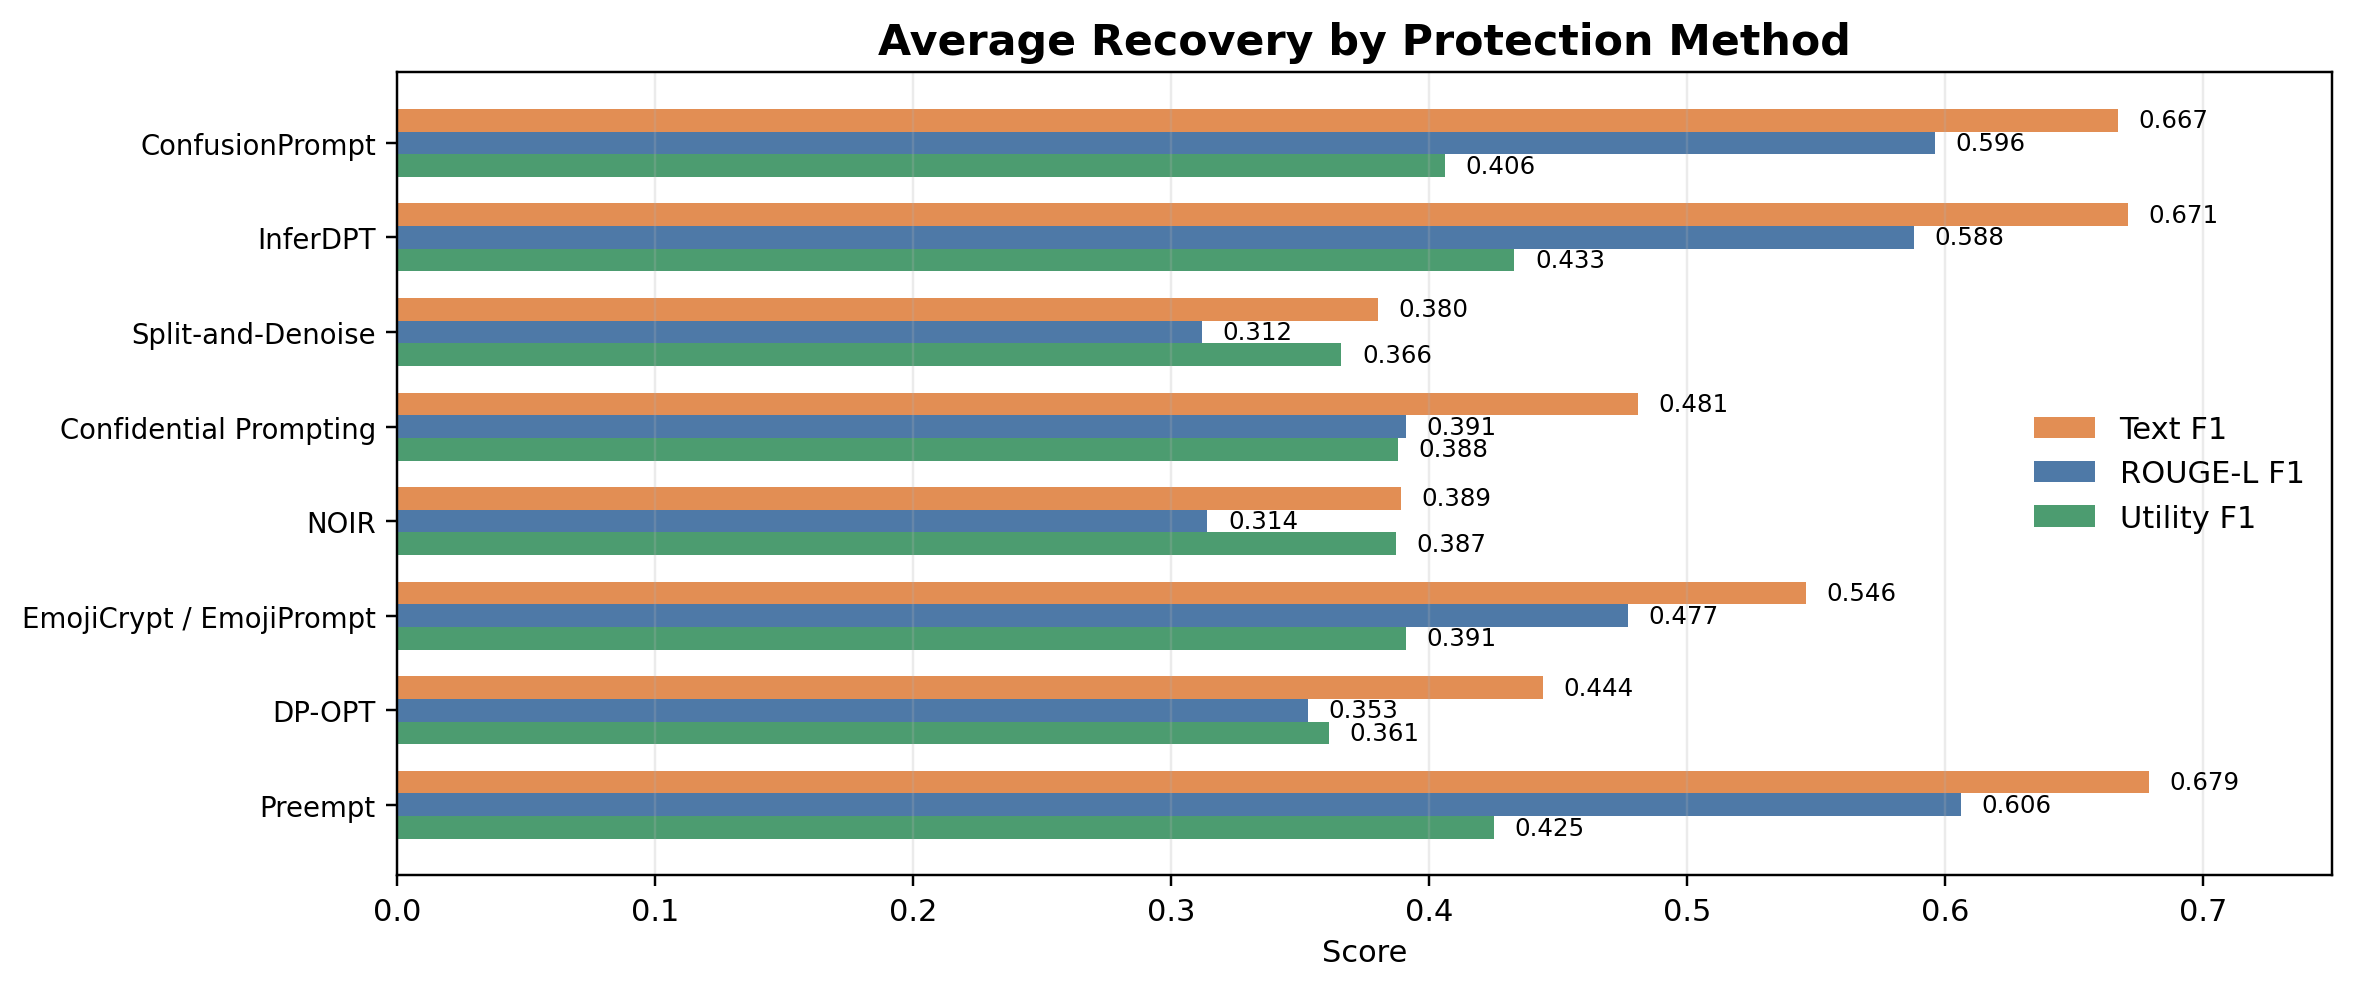
\includegraphics[width=0.95\linewidth]{figures/privacybench8_method_average.png}
    \caption{Average prompt-level held-out recovery across eight mechanism-aligned transformations.  Text F1 measures bag-of-token prompt overlap, ROUGE-L F1 measures sequential prompt overlap, and Utility F1 measures in-distribution behavior similarity on matched probes.}
    \label{fig:privacybench8_method_average}
\end{figure}

Pr$\epsilon\epsilon$mpt-style transformation has the highest average Text F1, 0.679, and ROUGE-L F1, 0.606, while InferDPT-style transformation has the highest average Utility F1, 0.433.  Split-N-Denoise-style has the lowest Text F1, 0.380, and ROUGE-L F1, 0.312; DP-OPT-style has the lowest Utility F1, 0.361.  All Utility F1 values remain nonzero, so the current recovery model constructs prompts that partially imitate cached behavior in every benchmark condition.  The differences cannot be attributed only to the original protection principles, because transformation fidelity, auxiliary metadata, and proxy traces also vary with our implementation.

Split-N-Denoise-style and DP-OPT-style have lower average Utility F1, 0.366 and 0.361.  One possible explanation is that their benchmark artifacts expose more abstract cues than token- or placeholder-based conditions.  This interpretation is descriptive rather than causal; an end-to-end ablation that holds all other evidence fixed is required to isolate the effect of representation type.

\subsection{Category-Level Recovery}

Figure~\ref{fig:privacybench8_utility_heatmap} shows Utility F1 by transformation and prompt category.  Averaged over transformations, Role/Persona is highest at 0.461, followed by Task Instruction at 0.411 and Context Knowledge at 0.409.  Constraints is lowest at 0.339, and Tool/Protocol reaches 0.359.  The category range is therefore larger than several method-to-method differences, indicating that prompt content is an important factor in recoverability.

\begin{figure}[t]
    \centering
    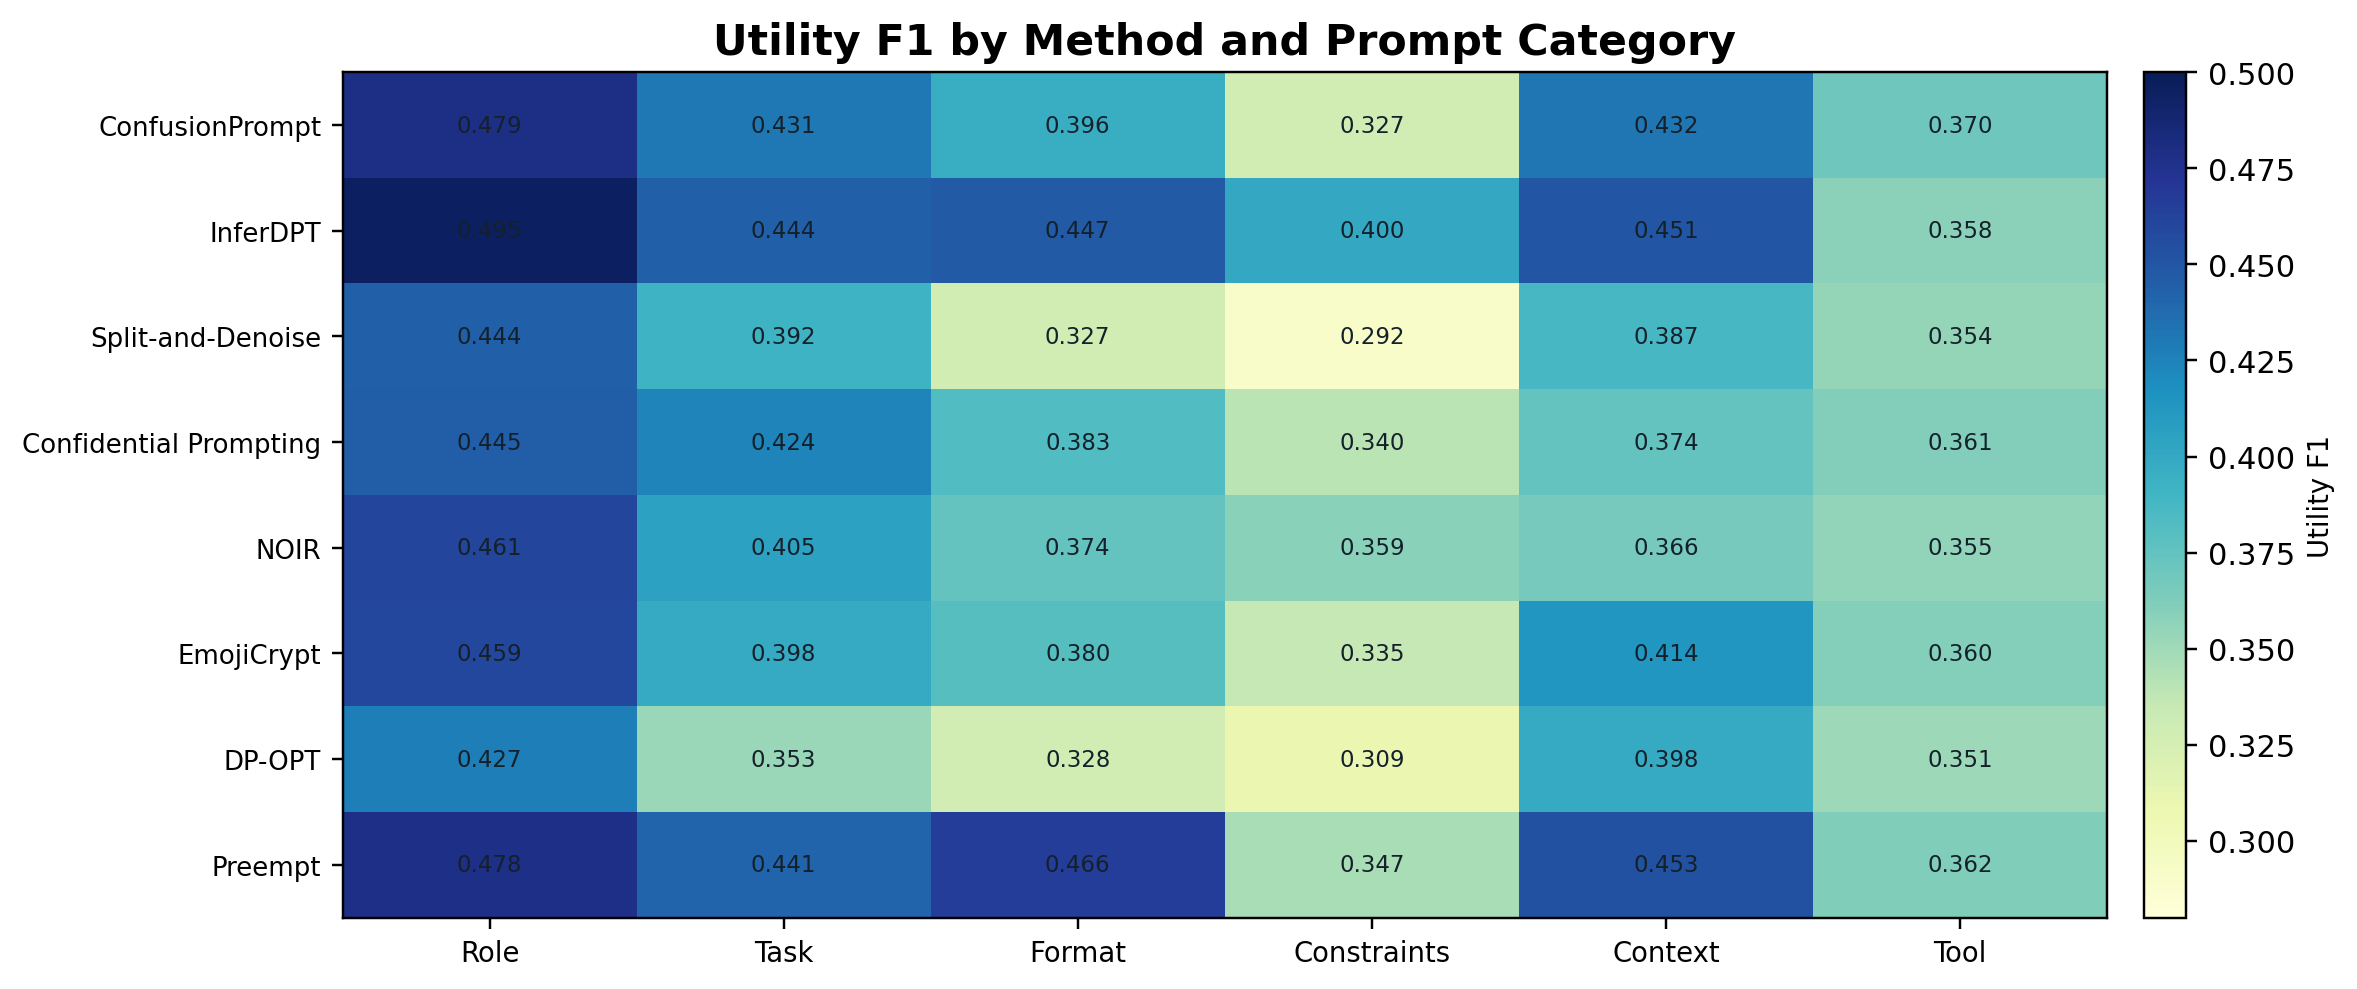
\includegraphics[width=0.95\linewidth]{figures/privacybench8_utility_heatmap.png}
    \caption{Utility F1 by mechanism-aligned transformation and prompt category.  Values use prompt-level held-out adapters but overlapping evidence/evaluation queries.}
    \label{fig:privacybench8_utility_heatmap}
\end{figure}

Role/Persona prompts are relatively recoverable because role instructions create repeated style, expertise, and identity patterns.  The category also benefits from explicit prompt labels and six-dimensional scores in the auxiliary metadata, so the result cannot be assigned to behavior traces alone.

Context Knowledge prompts are also relatively recoverable because the same background information can affect several outputs.  Repeated traces can expose this context even when its wording is transformed.

Constraints are harder because their behavior is sparse and conditional.  A rule may remain invisible unless a probe triggers a forbidden action, boundary case, or exception.  The current matched inputs follow the original task distribution but are not actively designed to trigger each rule.

Tool/Protocol prompts are also challenging because behavior can depend on exact argument names, step order, or API-like syntax.  Recovering a broad task description is insufficient when a small procedural error changes the output.

\section{Discussion}

\subsection{A Common Residual-Signal Hypothesis}

The benchmark supports a common hypothesis: a transformation that preserves function also preserves an output distribution shaped by the hidden instruction.  Confusion leaves genuine fragments, token perturbation retains semantically related words, sanitization retains types and templates, and symbolic representations retain encoded task cues.  These signals can complement behavior traces without requiring exact inversion of the transformation.

The present experiment does not isolate this behavior channel: it also supplies protected representations, semantic sketches, source metadata, and category scores.  The correct conclusion is therefore that the \emph{combined observable interface} contains recoverable signal.  Establishing that behavior alone is sufficient requires removing the other channels in a controlled ablation.

\subsection{Implications for Defense Evaluation}

These results motivate evaluating prompt protection with both representation-level and behavior-level privacy metrics.  A defense may reduce text similarity between \(p\) and \(T(p)\) while leaving role, task, format, context, or protocol information inferable from the observable interface.

Behavior-level evaluation is especially important for system prompts because their purpose is to shape model behavior.  This does not make utility-preserving defenses useless, nor does it invalidate formal privacy guarantees defined over a different sensitive object.  It means that evaluations and claims should distinguish exact-text secrecy, attribute privacy, representation privacy, and functional-structure privacy.

\subsection{Design Lessons}

The first lesson is that hiding prompt representation is not the same as hiding prompt behavior.  Future defenses should consider output-side leakage, not only input-side obfuscation.  The second lesson is that category-specific leakage matters.  Role and context information may leak through broad behavior patterns, while constraints and tool protocols may require targeted probes.  The third lesson is that semantic placeholders and sketches can still leak structure.  Sanitization and sketching reduce sensitive detail, but they often preserve task templates, field types, and interaction patterns.

A stronger defense may need adaptive routing, output filtering, behavior randomization, or query-budget limits in addition to prompt transformation.  However, each of these defenses introduces a new utility cost.  The central challenge is therefore not only how to hide the prompt, but how to hide the behaviorally useful structure of the prompt while preserving enough task performance.

\section{Conclusion}

We presented a system model, symbolic threat model, and reproducible multi-evidence recovery pipeline for studying functional-structure leakage from protected prompts.  Across eight mechanism-aligned transformations and six prompt categories, the common-interface benchmark obtains mean Text F1 between 0.380 and 0.679, ROUGE-L F1 between 0.312 and 0.606, and Utility F1 between 0.361 and 0.433.  These continuous scores show partial recovery of prompt wording and behaviorally useful structure without imposing a binary recovery threshold.

The main methodological lesson is that prompt privacy evaluation should specify the client-side private object and transformation state, the server-visible payload, side information, query transcript, and operational recovery criterion separately.  This separation also resolves the mutual-information ambiguity: responses add no conditional Shannon information once the complete server-visible payload, query, and model are known, although they can remain useful operational features for a bounded recovery procedure.  Table~\ref{tab:benchmark_scope} and the end-to-end protocol provide a common basis for extending the evaluation to complete protection systems.

\bibliographystyle{aaai2027}
\bibliography{prompt_protection_attack_refs}

\end{document}
